% Template for a Computer Science Tripos Part II project dissertation
\documentclass[12pt,a4paper,twoside,openright]{report}
\usepackage[pdfborder={0 0 0}]{hyperref}    % turns references into hyperlinks
\usepackage[margin=25mm]{geometry}  % adjusts page layout
\usepackage{graphicx, color}  % allows inclusion of PDF, PNG and JPG images
\usepackage{verbatim}
\usepackage{docmute}   % only needed to allow inclusion of proposal.tex
\usepackage{dsfont}
\usepackage{pdfpages}


\raggedbottom                           % try to avoid widows and orphans
\sloppy
\clubpenalty1000%
\widowpenalty1000%

\renewcommand{\baselinestretch}{1.1}    % adjust line spacing to make

%###########################################################################
\newcommand{\projectTitle}{Investigating the effect of \\
 & Translation Quality on Summarization Quality}                                        % more readable
 
 \newcommand{\red}[1]{\textcolor{red}{#1}}
 
 %###############################################################

\begin{document}

\bibliographystyle{plain}


%%%%%%%%%%%%%%%%%%%%%%%%%%%%%%%%%%%%%%%%%%%%%%%%%%%%%%%%%%%%%%%%%%%%%%%%
% Title


\pagestyle{empty}

\rightline{\LARGE \textbf{Martin Richards}}

\vspace*{60mm}
\begin{center}
\Huge
\textbf{\projectTitle}   \\[5mm]
Computer Science Tripos -- Part II \\[5mm]
Trinity Hall \\[5mm]
\today  % today's date
\end{center}

%%%%%%%%%%%%%%%%%%%%%%%%%%%%%%%%%%%%%%%%%%%%%%%%%%%%%%%%%%%%%%%%%%%%%%%%%%%%%%
% Proforma, table of contents and list of figures

\pagestyle{plain}

\chapter*{Proforma}

{\large
\begin{tabular}{ll}
Name:               & \bf Anish Das                      \\
College:            & \bf Trinity Hall                     \\
Project Title:      &  \projectTitle \\
Examination:        & \bf Computer Science Tripos -- Part II, June 2021  \\
Word Count:         & \bf \textcolor{red}{1587\footnotemark[1]
                      (well less than the 12000 limit)}  \\
Project Originator: & Dr Andrew Caines                  \\
Supervisor:         & Dr Andrew Caines \& Dr Zheng Yuan                   \\ 
\end{tabular}
}
\footnotetext[1]{This word count was computed
by \texttt{detex diss.tex | tr -cd '0-9A-Za-z $\tt\backslash$n' | wc -w}
}
\stepcounter{footnote}


\section*{Original Aims of the Project}

To investigate the effect of translation quality on summarization quality. To train Neural Machine Translation (NMT) models using the Transformer architecture for multiple languages and then applying a pre-trained state-of-the-art summarization model to the translations produced by the models. To find the correlation between the BLEU scores (translation metric) and the ROUGE scores (summarization metric). 

\red{[Finally, to try a different architecture for faster training of language models.]}

% To write a demonstration dissertation\footnote{A normal footnote without the
% complication of being in a table.} using \LaTeX\ to save
% student's time when writing their own dissertations. The dissertation
% should illustrate how to use the more common \LaTeX\ constructs. It
% should include pictures and diagrams to show how these can be
% incorporated into the dissertation.  It should contain the entire
% \LaTeX\ source of the dissertation and the makefile.  It should
% explain how to construct an MSDOS disk of the dissertation in
% Postscript format that can be used by the book shop for printing, and,
% finally, it should have the prescribed layout and format of a diploma
% dissertation.


\section*{Work Completed}

The Transformer architecture was built from scratch and has been used to create multiple translation models. Translation models have been used to translate the documents in the evaluation gv-crowd dataset from \cite{nguyen-daume-iii-2019-global}. The translated sentences were then summarized. The BLEU and ROUGE metrics were calculated along with qualitative comparison of the two scores.

\section*{Special Difficulties}

\red{Learning how to training Transformers is a difficult task that requires proper care towards various factors. \\
And having to work remotely for the entire year.} 
 
\newpage
\section*{Declaration}

I, Anish Das of Trinity Hall, being a candidate for Part II of the Computer Science Tripos, hereby declare 
that this dissertation and the work described in it are my own work,
unaided except as may be specified below, and that the dissertation
does not contain material that has already been used to any substantial
extent for a comparable purpose.

\bigskip
\leftline{Signed [signature]}

\medskip
\leftline{Date [date]}

\tableofcontents

\listoffigures

\newpage
\section*{Acknowledgements}

A huge thanks to my supervisors, Andrew Caines and Zheng Yuan, who's support throughout the project was immense. 

%%%%%%%%%%%%%%%%%%%%%%%%%%%%%%%%%%%%%%%%%%%%%%%%%%%%%%%%%%%%%%%%%%%%%%%
% now for the chapters

\pagestyle{headings}

\chapter{Introduction}

\section{Overview of the files}

This document consists of the following files:

\begin{itemize}
\item \texttt{makefile} --- The makefile for the dissertation and
                         Project Proposal
\item \texttt{diss.tex} --- The dissertation
\item \texttt{proposal.tex}  --- The project proposal 
\item \texttt{figs} -- A directory containing diagrams and pictures
\item \texttt{refs.bib} --- The bibliography database
\end{itemize}

\section{Building the document}

This document was produced using \LaTeXe which is based upon
  To build the document you first need to
generate \texttt{diss.aux} which, amongst other things, contains the
references used.  This if done by executing the command:

\texttt{pdflatex diss}

\noindent
Then the bibliography can be generated from \texttt{refs.bib} using:

\texttt{bibtex diss}

\noindent
Finally, to ensure all the page numbering is correct run \texttt{pdflatex}
on \texttt{diss.tex} until the \texttt{.aux} files do not change.  This
usually takes 2 more runs.

\subsection{The makefile}

To simplify the calls to \texttt{pdflatex} and \texttt{bibtex}, 
a makefile has been provided, see Appendix. 
It provides the following facilities:

\begin{description}

\item\texttt{make} \\
 Display help information.

\item\texttt{make proposal.pdf} \\
 Format the proposal document as a PDF.

\item\texttt{make view-proposal} \\
 Run \texttt{make proposal.pdf} and then display it with a Linux PDF viewer
 (preferably ``okular'', if that is not available fall back to ``evince'').

\item\texttt{make diss.pdf} \\
 Format the dissertation document as a PDF.

\item\texttt{make count} \\
Display an estimate of the word count.

\item\texttt{make all} \\
Construct \texttt{proposal.pdf} and \texttt{diss.pdf}.

\item\texttt{make pub} \\ Make \texttt{diss.pdf}
and place it in my \texttt{public\_html} directory.

\item\texttt{make clean} \\ Delete all intermediate files except the
source files and the resulting PDFs. All these deleted files can
be reconstructed by typing \texttt{make all}.

\end{description}


\section{Counting words}

An approximate word count of the body of the dissertation may be
obtained using:

\texttt{wc diss.tex}

\noindent
Alternatively, try something like:

\verb/detex diss.tex | tr -cd '0-9A-Z a-z\n' | wc -w/


\chapter{Preparation}

This chapter is empty!


\chapter{Implementation}

\section{Verbatim text}

Verbatim text can be included using \verb|\begin{verbatim}| and
\verb|\end{verbatim}|. I normally use a slightly smaller font and
often squeeze the lines a little closer together, as in:

{\renewcommand{\baselinestretch}{0.8}\small
\begin{verbatim}
GET "libhdr"
 
GLOBAL { count:200; all  }
 
LET try(ld, row, rd) BE TEST row=all
                        THEN count := count + 1
                        ELSE { LET poss = all & ~(ld | row | rd)
                               UNTIL poss=0 DO
                               { LET p = poss & -poss
                                 poss := poss - p
                                 try(ld+p << 1, row+p, rd+p >> 1)
                               }
                             }
LET start() = VALOF
{ all := 1
  FOR i = 1 TO 12 DO
  { count := 0
    try(0, 0, 0)
    writef("Number of solutions to %i2-queens is %i5*n", i, count)
    all := 2*all + 1
  }
  RESULTIS 0
}
\end{verbatim}
}

\section{Tables}

\begin{samepage}
Here is a simple example\footnote{A footnote} of a table.

\begin{center}
\begin{tabular}{l|c|r}
Left      & Centred & Right \\
Justified &         & Justified \\[3mm]
%\hline\\%[-2mm]
First     & A       & XXX \\
Second    & AA      & XX  \\
Last      & AAA     & X   \\
\end{tabular}
\end{center}

\noindent
There is another example table in the proforma.
\end{samepage}

\section{Simple diagrams}

Simple diagrams can be written directly in \LaTeX.  For example, see
figure~\ref{latexpic1} on page~\pageref{latexpic1} and see
figure~\ref{latexpic2} on page~\pageref{latexpic2}.

\begin{figure}
\setlength{\unitlength}{1mm}
\begin{center}
\begin{picture}(125,100)
\put(0,80){\framebox(50,10){AAA}}
\put(0,60){\framebox(50,10){BBB}}
\put(0,40){\framebox(50,10){CCC}}
\put(0,20){\framebox(50,10){DDD}}
\put(0,00){\framebox(50,10){EEE}}

\put(75,80){\framebox(50,10){XXX}}
\put(75,60){\framebox(50,10){YYY}}
\put(75,40){\framebox(50,10){ZZZ}}

\put(25,80){\vector(0,-1){10}}
\put(25,60){\vector(0,-1){10}}
\put(25,50){\vector(0,1){10}}
\put(25,40){\vector(0,-1){10}}
\put(25,20){\vector(0,-1){10}}

\put(100,80){\vector(0,-1){10}}
\put(100,70){\vector(0,1){10}}
\put(100,60){\vector(0,-1){10}}
\put(100,50){\vector(0,1){10}}

\put(50,65){\vector(1,0){25}}
\put(75,65){\vector(-1,0){25}}
\end{picture}
\end{center}
\caption{A picture composed of boxes and vectors.}
\label{latexpic1}
\end{figure}

\begin{figure}
\setlength{\unitlength}{1mm}
\begin{center}

\begin{picture}(100,70)
\put(47,65){\circle{10}}
\put(45,64){abc}

\put(37,45){\circle{10}}
\put(37,51){\line(1,1){7}}
\put(35,44){def}

\put(57,25){\circle{10}}
\put(57,31){\line(-1,3){9}}
\put(57,31){\line(-3,2){15}}
\put(55,24){ghi}

\put(32,0){\framebox(10,10){A}}
\put(52,0){\framebox(10,10){B}}
\put(37,12){\line(0,1){26}}
\put(37,12){\line(2,1){15}}
\put(57,12){\line(0,2){6}}
\end{picture}

\end{center}
\caption{A diagram composed of circles, lines and boxes.}
\label{latexpic2}
\end{figure}



\section{Adding more complicated graphics}

The use of \LaTeX\ format can be tedious and it is often better to use
encapsulated postscript (EPS) or PDF to represent complicated graphics.
Figure~\ref{epsfig} and~\ref{xfig} on page \pageref{xfig} are
examples. The second figure was drawn using \texttt{xfig} and exported in
{\tt.eps} format. This is my recommended way of drawing all diagrams.


\begin{figure}[tbh]
\centerline{
\includegraphics{figs/cuarms.pdf}}
\caption{Example figure using encapsulated postscript}
\label{epsfig}
\end{figure}

\begin{figure}[tbh]
\vspace{4in}
\caption{Example figure where a picture can be pasted in}
\label{pastedfig}
\end{figure}


\begin{figure}[tbh]
\centerline{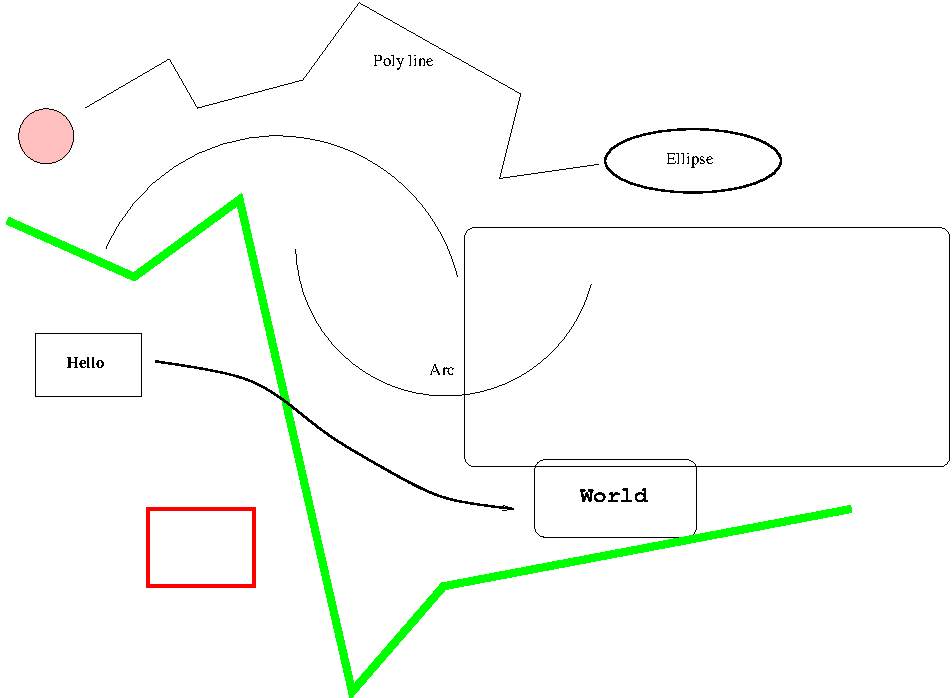
\includegraphics{figs/diagram.pdf}}
\caption{Example diagram drawn using \texttt{xfig}}
\label{xfig}
\end{figure}


\chapter{Evaluation}

\section{Printing and binding}

Use a ``duplex'' laser printer that can print on both sides to print
two copies of your dissertation. Then bind them, for example using the
comb binder in the Computer Laboratory Library.

\section{Further information}

See the Unix Tools notes at

\url{http://www.cl.cam.ac.uk/teaching/current-1/UnixTools/materials.html}


\chapter{Conclusion}

I hope that this rough guide to writing a dissertation is \LaTeX\ has
been helpful and saved you time.


%%%%%%%%%%%%%%%%%%%%%%%%%%%%%%%%%%%%%%%%%%%%%%%%%%%%%%%%%%%%%%%%%%%%%
% the bibliography
\addcontentsline{toc}{chapter}{Bibliography}
\bibliography{refs}

%%%%%%%%%%%%%%%%%%%%%%%%%%%%%%%%%%%%%%%%%%%%%%%%%%%%%%%%%%%%%%%%%%%%%
% the appendices
\appendix

% \chapter{Latex source}

% \section{diss.tex}
% {\scriptsize\verbatiminput{diss.tex}}

% \section{proposal.tex}
% {\scriptsize\verbatiminput{proposal.tex}}

% \chapter{Makefile}

% \section{makefile}\label{makefile}
% {\scriptsize\verbatiminput{makefile.txt}}

% \section{refs.bib}
% {\scriptsize\verbatiminput{refs.bib}}


\chapter{Project Proposal}

\documentclass[12pt, a4paper]{article}
\usepackage[utf8]{inputenc}
\usepackage{graphicx}
\usepackage[margin=1.25in]{geometry}
\usepackage{hyperref}
\usepackage[
backend=biber,
style=alphabetic,
sorting=ynt
]{biblatex}
\usepackage{dsfont}
\usepackage{pdfpages}

% \newcommand{\boldItem}[2]{\item \textbf{#1} \textit{(#2)}  -\\}

\title{ Computer Science Part II Project Proposal\\
Investigating the effect of Translation on Summarization quality}
\author{Anish Das}
\date{\today}

\addbibresource{proposal.bib}

\begin{document}

% \includepdf{try2.pdf}

% \maketitle


\subsection*{Introduction}
Cross-Lingual Summariation (CLS) aims to produce a summary in a target language from a document in a different source language. This allows people who are fluent in the target language to get the salient details in an article written in foreign languages. In the Cross-Lingual Summarization there are two main steps: 1) translate and then 2) summarize, which introduces the problem of propagation of errors from the translation step to the summarization step.

The motivation behind such a system is that there are many news articles being published around the world which are not accessible to everyone because of the language barrier. Machine Translation helps alleviate this problem, by using statistical methods and neural networks to produce high quality translation without any human intervention. 
However, the amount of textual material i.e.news articles and blog posts is immense and it continues to grow everyday. With the sheer amount of material to cover people have to resort to searching for keywords and skimming through the results. Automatic Text Summarization allows us to extract the salient details in the text and then join them together to form one cohesive summary. 

This project aims to investigate the effect of bad translation on the summary that is produced. Since CLS is a two step process, any error in the first step should be propagated to the next. Moreover, we don't have sufficient resource to train a state-of-the-art Machine Translation system for every language . This means that the translation produced by the low-resource languages will have some inaccuracies in them.

\subsection*{Resource Declaration}
I plan to use my own computer (2 GHz-4 Cores; 8 GB RAM; 128 GB SSD \& 1TB HDD; Windows10-Home). I plan on maintaining a backup folder on GitHub and External HDD daily while also using Google Backup and Sync to continuously backup my device to protect against failure. I am not using any paid service and all datasets used are readily available and free to use therefore, in case of failure, I would like to move to an MCS machine where I would be able to commence my work with only a slight delay.
\\
\textbf{Special Resource required}
To train the machine learning models access to HPC is requested. 
\\
For development: PyTorch, Moses, \textbf{TBD}
\\
The datasets used will be: 
\begin{itemize}
  \item Summarization: CNN/Daily Mail dataset (\href{https://github.com/abisee/cnn-dailymail}{CNN/Daily Mail-link})
  \item Evaluation: gv-summaries dataset created by the authors. (Gotten after filling the \href{https://github.com/abisee/cnn-dailymail}{google form} available on their paper: \href{https://forms.gle/gpkJDT6RJWHM1Ztz9}{Form-link})
  \item Translations: News-Commentary dataset(\href{http://opus.nlpl.eu/News-Commentary-v11.php}{NCv11-link}) and the ParaCrawl dataset (\href{http://opus.nlpl.eu/ParaCrawl.php}{ParaCrawl-link}) for langauges French, Spanish and German.
\end{itemize}
 

\subsection*{Starting Point}
This project will re-do the experiments done by \textit{Khanh Nguyen and Hal Daumé III in their paper "Global Voices: Crossing Borders in Automatic News Summarization"} with a few alterations and will be starting from scratch for the translators. I have not written any code related to this project. \\
In terms of relavent course work, I have done the Scientific Computing (from Part 1A) and Artificial Intelligence (from Part 1B) which served as a base for a further MIT Deep Neural Network course I took which had 1 lecture on NLP/Sequence Modelling. \\
I will be using a pre-trained Summarization tool which need to be specially trained for this task. I have located the dataset to be used but have only downloaded the gv-summaries dataset.   

\subsection*{Substance and Structure of the Project}

\subsubsection*{Baselines}
\begin{itemize}
  \item FIRST50: copies the first 50 words of the English version of the Source Article.
  \item PEFECT-TRANS: using the perfect translations from the gv dataset to produce summaries.
  \item TRANS-THEN-SUM: Translating using the models trained and then summarizing.
\end{itemize}

\subsubsection*{Core} 

In the paper from which this idea has been borrowed they use languages of different resource availability (i.e. if there are a large volume of parallel aligned sentences then we have a high-resource language pair and because of the large amounts of data our model will perform better and vice versa) to investigate whether the quality of translation affect the summaries produced. I am extending it further by saving the features of the translator model while it is in training so as to have a few worse translation models for the same language that output inferior translations. This differs from what they did in the paper because they used languages of different resource availability. %I believe the language you are translating from can have an impact on the summarization and would like to discover if my intuition is correct. 
\\
Therefore, I have chosen French, German and Spanish as the source languages and the target language is English. All of the translation models will be sentence-level models. 
%For this CLS task, all the translators will have the target language English and the summarizer will be a monolingual translator which takes and returns text in English. All the translation models will be sentence-level translators. 
\\
Therefore the Core of the project can be broken down into the following steps which need to follow this order to save time and for smooth functioning: 
\begin{enumerate}
  
  \item Research about transformers/summarizers
  \item Build and test the Transformer
  \item Normalize the datasets before training
  \item Build/train the Summarization tool.
  \item Evaluate the Core part of the project.
  \item Evaluate feasibility of extensions and start working on them.
  \item Write dissertation. 
  
\end{enumerate}
However, we want the Summarization tool to be good so that it doesn't introduce any errors. Therefore, initially I am going to use a pre-trained Summarization tool which will be further trained for this task. This is also a way to manage risk since the translation models could take a long time to train.

\subsubsection*{Extensions}
Once the core part of the project is complete, in order to build a better understanding of the effect of translation on summarization I think these would be some good extensions: 
\begin{enumerate}
  \item Train translators for more languages and perform qualitative evaluation on them as well
  \item Learn about, build, test and train more Summarization tools
\end{enumerate} 

For the new language part, they will be chosen from the ParaCrawl/News-Commentary dataset. 


\subsection*{Evaluation}
I will be using two metrics for this task: BLEU and ROUGE. In general BLEU measures precision i.e. how many of the words in the machine generated text are present in the reference text while ROUGE measures recall i.e. how many of the words in the reference text are present in the generated text. Usually, BLEU is used for assessing translation quality while ROUGE is used for summarization quality.

\subsubsection*{BLEU}
To evaluate the translation produced the BLEU (Bilingual Evaluation Understudy) is used. The better the machine translation's output, the closer it will be to the human translation of the same piece of text, and this forms the central idea for BLEU. Scores are calculated for segments - usually sentences - by comparing them to a set of good translations. These scores are then averages for the corpus or the document to get the estimate for the quality. Note: readability and correctness are not taken into account. The scores produced are between 0 and 1 (inclusive)

\subsubsection*{ROUGE}
ROUGE or Recall-Oriented Understudy for Gisting Evaluation is a set of metrics for evaluating automatic summarization tools. They compare the summaries produced to a set of reference summaries available. 
\begin{itemize}
  \item \textbf{ROUGE-N:} overlap of N-grams in the output and reference summaries. 
  
  \item \textbf{ROUGE-L:} Longest common subsequence(LCS) based statistics. 
  
  \item \textbf{ROUGE-W:} Weighted LCS-based statistic that will favor consecutive LCSes.
  
  \item \textbf{ROUGE-S:} Skip-bigram based co-occurence statistic.
  
  \item \textbf{ROUGE-SU:} Skip-bigram and unigram-based statistic. 
\end{itemize}

\subsubsection*{F Measure}
This is the final metric that will used to compare the summaries against each other. Using the BLEU metric we will have a decent idea about the quality of the translations. The reference summaries shall be gv-crowd (crowd sourced summaries) and gv-snippet (a catchy summary of the article meant to draw people in) using the F Measure metric. At the end we will have evaluated the gv summaries against the ones produced by the baselines mentioned above. 

\subsection*{Success Criterion}
%\textit{Explain the BLUE and ROUGE metrics these will be expanded upon}
As described above the translation quality will be evaluated using the BLEU metric. The summaries produced will be evaluated on their own using the ROUGE-* metric. Finally, when comparing two summaries i.e. the summaries produced to the reference summary we will use F-Measure where the Precision will be the BLEU metric and Recall will be different ROUGE-* metrics. 

\subsubsection*{Core}
\begin{itemize}
  \item Translators have been implemented
  \item Summarizer has been implemented
  \item A qualitative comparison of the performance of the different summaries produced and the baselines.
\end{itemize}

\subsubsection*{Extensions}
The following criteria define the success in the extension tasks:
\begin{itemize}
  \item Translator for new language is implemented/trained and quantitative evaluation has been conducted.
  \item New summarization models have been implemented and further quantitative evaluation has been conducted.
\end{itemize}


\subsection*{Concepts}
There are two main types of models that will be developed - Translation model using Transformer and Summarization model. 

\subsubsection*{Feed-Forward Neural Network}
The most basic form of an Artificial Neural Network which is meant to mimic the neural connections in the brain and can be used to compute any function. The most basic part of a neural net is the perceptron. It takes in a number of Real ($\mathds{R}$) values and performs a weighted sum to an already existing bias value. The sum is then passed through an activation functions usually sigmoid (\( \sigma(x) = \frac{1}{1 + e^{-x}} \)) or tanh. Activation functions should be continuous and differentiable, and it is chosen to suite the problem. The output from the activation function is the output for the perceptron. \\
\\
Multiple percetrons with the same input size form a layer and multiple layers from a Neural Network. We generally have weights matrices which store the weights for the weighted sum operation for each perceptron. \\  
Therefore, the trainable features of a Neural Network are the weights matrices and the biases for each perceptron which can be optimized to then simulate any function. 

\subsubsection*{Back-propagation}
The widely used algorithm to train Neural Networks is back-propagation algorithm. There are many optimizations that exists for this process but this covers the basic idea behind training a Neural Network. \\\\
Using the loss function we will have evaluated our error for the network. We then proceed to compute the partial derivative of this error for each weight and bias in the network. And for each batch of the training we aggregate and scale these values to get the value to be added to the features (weights and biases) to make the network better. \\
We continue this process until we see there is no improvement in the error value. 

\subsubsection*{Self-Attention}
Self attention is a sequence-to-sequence operation i.e. a sequence of vectors of length T go in and we get a sequence of vectors of length T as well. Suppose our input vectors are \( I_1, I_2, ... I_T \) and the self-attention outputs are: \( O_1, O_2,... O_T \), then

\[ O_i = \sum_j w_{ij} * I_j\] 
where \( w'_{ij} = I_i^T * I_j\) and we get \(w_{ij}\) by using softmax.

\subsubsection*{Queries, Keys and Values}
Each input vector $I_i$ is used in 3 different ways:
\begin{enumerate}
  \item Query: Compared to every other weight to form the weights for $O_i$
  \item Key: Used to form the weights for every other vector $O_j$
  \item Value: Finally used in the weighted sum for the final output vectors.
\end{enumerate}

Here we add 3 more K x K weight matrices (where K is the input/output vector dimension) \( W_q, W_k , W_v\) to compute:
\begin{center}
\(q_i = W_q x_i\) \textrm{and}  \(k_i = W_k x_i\) \textrm{and}  \(v_i = W_v x_i\)
\end{center}
and then
\[w'_{ij} = q_i^T * k_i\]
\[w_{ij} = softmax(w'_{ij})\]
\[O_i = \sum_j w_{ij} * I_j\]

Now that we have added a step in between by introducing the attention heads we can add more attention head that can potentially be trained to have greater discrimination power. This is called Multi-head Attention.

\subsubsection*{Transformer Architecture - Encoder}
The first layer in a Transformer Architecture is the self-attention layer however, once we pass through the self-attention layer we loose all spacial information about where each word was located. In order to counter this problem a vector containing multiple sine/cosine waves at different frequencies are used. This allows the transformer to reason about the position of each word. \\
Following the Self-attention layer there is a Feed-Forward layer that generates the encoded vectors. Once all the tokens have been passed through the transformer we start Decoding. Note: There may be more encoding steps which will take the current output and repeat. 

\subsubsection*{Transformer Architecture - Decoder} 
The output from the top encoder is used to form the form the encoder-decoder attention layer's \(W_k\)  \textrm{and}  \(W_v\) matrix and it takes the Queries matrix from the encoder's self-attention layer. \\
Input to the Decoder is a special symbol at the start and after that is the previous output, such that it can see what has been predicted before. The first layer is again a self-attention layer. The output from this layer is normalized and then it moves into the Encoder-Decoder Attention layer. Output from there is directed to a Feed-Forward layer. After which all the data is passed to a Linear layer. Finally, a softmax function provides the probability of next word from our corpus.

\subsubsection*{Automatic Summarization}
There are two way to go about summarizing a piece of text: 1) Extraction, or 2) Abstraction. Extractive summaries employ statistical methods to identify important or the salient sections of text and copying them. Abstractive Summaries aim to interpret the material before generating a summary which are shorter and convey significantly more information. Extractive summaries produce better result because they don't need to worry about grammatical correctness since they are afterall copying the text, however, they do fall into the trap of repeating themselves or not picking up on some important points. Abstractive summaries do a better job of picking the important points, however, lack in readability, and most abstractive summaries have to have some form of extractive step in them as well.   


\subsection*{Work Plan and Timetable}
 
The preliminary plan is split into 2/3 week components starting after the project proposal deadline. Please note that these are just estimates and the Plan will need to be changed if certain components are failing. However, in the interest of saving time, I am undertaking the implementation of the Transformer for the translator before everything else (like examining datasets) since the training can happen parallel to the dataset examination step. Similarly, the work on the Summarization tool is the third item on the overall plan. 
 
\subsubsection*{Timetable}
\begin{enumerate}
  \item {\textbf{24th Oct - 7th Nov}} \textit{2 weeks}  -\\ Research on, and understand Transformers and associated concepts along with Summarization models/methods. Gain familiarity with PyTorch
  
  \item \textbf{{8th Nov - 28th Nov}} \textit{3 weeks}   -\\
  Begin building the Transformer, and then test the implementation.
  
  \item \textbf{{29th Nov - 19th Dec}} \textit{3 weeks}   -\\
  Normalize the dataset if necessary. \\
  Continue working on the Transformer. \\
  Begin work on the Summarizer.
  
  \item \textbf{{20th Dec - 9th Jan}} \textit{3 weeks}  -\\ 
  Aim to finish the programming work related the main Transformer architecture during the vacation.\\ 
  Should also re-evaluate the feasibility of the extensions.
  
  \item \textbf{{10th Jan - 23rd Jan}} \textit{2 weeks}   -\\
  Begin training of the Transformer. \\ Continue working on the summarization tool.
  
  \item \textbf{{24th Jan - 6th Feb}} \textit{2 weeks}   -\\
  Start building a pipeline using the translator and summarization tool for evaluation and perform some preliminary qualitative assessment. \\
   If possible start the dissertation.
  
  \item \textbf{{7th Feb - 20th Feb}} \textit{2 weeks}   -\\
  Make a drat/plan for the dissertation. \\ 
  Start working on the extensions. \\
  Extensions will include finding relevant datasets for training the Translators and/or building more Summarization tools.
  
  \item \textbf{{21st Feb - 6th Mar}} \textit{2 weeks}  -\\
  start work on introduction and preparation chapters\\
  Continue working on the extensions.
  
  \item \textbf{{7th Mar - 20th Mar}} \textit{2 weeks}  -\\
  Start work on Implementation chapter.\\
  Send first two chapters for review to Supervisor(Andrew Caines) and DoS (Simon Moore)
  
  \item \textbf{{21st Mar - 3rd April}} \textit{2 weeks}  -\\
  Finish working on extensions. \\
  Start working on evaluation and conclusion chapters.
  Send in Implementation chapter for review.
  
  \item \textbf{{4th April - 17th April}} \textit{2 weeks}  -\\
  Send in last few chapters for review.
  
  \item \textbf{{18th April - 1st May}} \textit{2 weeks}  -\\
  complete and review the dissertation.
\end{enumerate}

% \printbibliography
\end{document}


\end{document}